In this section, we demonstrate the applicability of the proposed ICDF-based approach in two case studies of the microgrid operation. The properties and performance were investigated using streamed signals from the IoT devices. The successful deployment indicates that our approach is suitable for existing alerting mechanisms of process automation infrastructure.

The case studies were realized using Python 3.10.1 on a MAC with an M1 CPU and 8 GB RAM. The percent point function was solved using an iterative root-finding algorithm, Brent's method.

\subsection{Battery Energy Storage System (BESS)}\label{AA:Case1}
First, we verify our proposed method on BESS. Tight control of the battery cell temperature is needed for the optimal performance and maximum lifespan of the battery. Identifying anomalous events and removal of corrupted data might yield significant improvement on the process control level.

The sampling rate of the signal measurement is 1 minute. However, network communication is prone to packet dropout, which results in non-uniform sampling. To protect the sensitive business value of the data, we normalize all signals to the range $[0, 1$]. The goal is to mark anomalous events in the data and provide adaptive process limits from the self-learning model.

Fig. \ref{fig:threshold} renders measurement of average battery cell temperature from 21\textsuperscript{st} February until 26\textsuperscript{th} March. We can observe multiple anomalies of various sources given this span, for instance, packet dropout, suspicious events, intermittent sensor failure, and change points in data distribution. Dates of observation given the listed events will be provided later in the paper.

\begin{figure}[htbp]
 \centerline{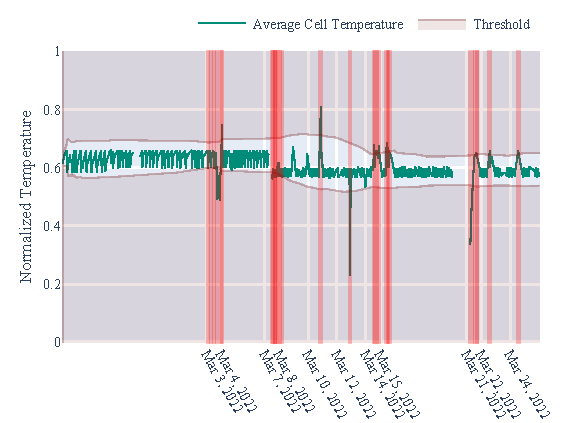
\includegraphics{figures/Average_Cell_Temperature_168_hours_sliding_thresh.pdf}}
 \caption{Time Series of Average Battery Cell Temperature measurement (green line) and predicted anomalous events (red vertical rectangles). The reddish fill bonded by the red line represents an area of anomalous behavior as given by the anomaly detector.}
 \label{fig:threshold}
\end{figure}

The user-defined parameters were set to 7 days for the expiration period and 5 hours for the time constant. Anomalies found during the first day of the service are ignored due to the initialization of the detector. In this case study, the anomaly detection problem was approached by the online model fitting based on Subsection \ref{train}

Using the online prediction described in Subsection \ref{predict} we tag the sample as the anomaly or normal data point. Fig. \ref{fig:threshold} renders red vertical rectangles over the regions from the start until the end of the predicted anomalous event.

The results on Average Cell Temperature in Fig. \ref{fig:threshold} show that the model could capture anomalous patterns of various sources. Despite self-learning without supervision, the model-classified anomalies were also confirmed by the data provider after inspection. For instance, a rare event of manipulation with BESS on 3\textsuperscript{rd}, followed by peak on 4\textsuperscript{th} March. BESS relocation on 7\textsuperscript{th}, led to a change point which was alerted and the system adapted completely over the course of 1 day. Calibration resulted in peak values through 10\textsuperscript{th} to 15\textsuperscript{th} March, and faulty measurements on the 12\textsuperscript{th} March followed by a packet loss on 21\textsuperscript{st} March were alerted too. The system tagged the next two tests of temperature control switch-offs.

The model's ability to detect anomalous behavior is crucial for effective dynamic process thresholding. The real-valued threshold mechanism, described in Subsection \ref{constrait}, provided up-to-date upper and lower bounds for the signal bounds. The model accurately detected breakouts from the range, as illustrated in Fig. \ref{fig:threshold}. The system adapted quickly to a change point on March 7\textsuperscript{th} and mitigated the effects of anomalies on the signal distribution. The user-defined parameters $t_e$ and $t_c$ govern the speed of adaptation and the tightness of the limits.

\subsection{Power Inverter}\label{AA:Case2}
A second case study demonstrates the proposed method's applicability to the temperature of the power inverter. During high load periods, inverters can heat up swiftly. Technical documentation of every inverter provides details on continuous output rating as a function of temperature that implies static process limits. Normally, for high temperatures, the rating drops rapidly. Nevertheless, the impact of aging and ambient conditions may render conservative limits impractical. Thus the alerting mechanism for the detection of abnormal heating shall be developed. Providing a real-valued anomaly threshold tightens the theoretical operating conditions and gives the ability to track the performance and deviations.

\begin{figure}[htbp]
\centerline{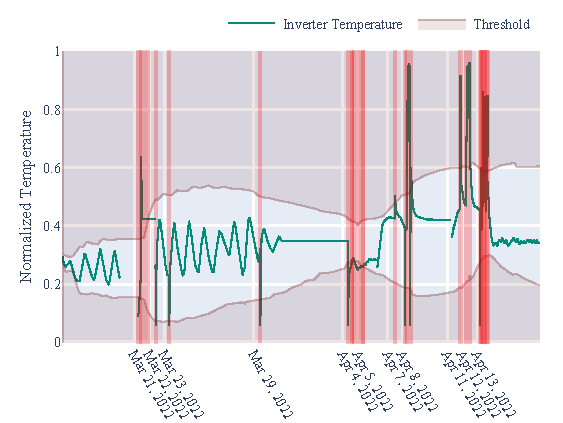
\includegraphics{figures/Inverter_Temperature_168_hours_sliding_thresh.pdf}}
\caption{Time Series of Inverter Temperature measurement (green line) and predicted anomalous events (red vertical rectangles). The reddish fill bonded by the red line represents an area of anomalous behavior.}
\label{fig:cs2_threshold}
\end{figure}

Fig. \ref{fig:cs2_threshold} depicts one month of operation of the inverter from 16\textsuperscript{th} March to 17\textsuperscript{th} April 2022. After the packet loss before 21\textsuperscript{st} March, rare temperature events occurred. Both events fell out of the normal operating conditions given by the dynamic process limit. Four faulty sensor readings follow from 22\textsuperscript{nd}, 23\textsuperscript{rd}, 29\textsuperscript{th} March and 4\textsuperscript{th} April. The first two are tagged as anomalies, though almost missed due to the prolonged data loss. If $t_e$ is not fully reached, the self-learning algorithm uses anomalies for updating, indicating the need for a shorter grace period to prevent false positives. The third faulty reading was tagged without influencing the distribution and operational boundaries due to the effect of $t_c$. Oscillations, that kept the boundaries relaxed vanished after 29\textsuperscript{th} March, which further tightened the process limit range. After the fourth caught fault, which was not used to update the model, the detector deliberately adapted the range of normal operation during the next day. Outliers during the sensors rescaling period from 7th April were all tagged. However, the relaxed operational conditions would probably lead to ignorance of smaller anomalous oscillations in a given period.

Lastly, Fig. \ref{fig:comparison} provides a comparison with other methods routinely used for online anomaly detection, namely, Half-Space Trees (Trees) and One-class SVM (OSVM). The detection is performed using default model parameters and a tuned quantile filter using grid search for the selection of anomalous scores. The ICDF-based method brings improved adaptation to changing conditions, retaining a low false positive rate.
\begin{figure}[htbp]
 \centerline{\includegraphics{../compare_inv_univariate_h50.pdf}}
 \caption{Time Series of Inverter Temperature measurement (green line) and predicted anomalous events (red vertical rectangles) for Half-Spaced Trees (Trees), One-class SVM (OSVM), and proposed method (ICDF).}
 \label{fig:comparison}
\end{figure}
